
\subsection{2.3. Энергия ионной кристаллической решетки. Взаимосвязь природы ионов и свойств кристаллов. (Приведите не менее двух разных типов кристаллических решеток, сравните их).} 

\par\bigskip
	
Уравнение для взаимодействия одной пары ионов (отрицательно и
положительно заряженных):

$$E=\frac{z^+z^-\bar{e}^2}{4\pi\varepsilon_0r_0}$$

\begin{center}
$r_0$ - расстояние
\par\smallskip
$\varepsilon_0$ - диэл. постоянная
\par\smallskip
$\bar{e}$ - заряд электрона
\par\smallskip
$z^\pm$ - величины зарядов ионов
\end{center}

Естественно, что это уравнение не учитывает все взаимодействия в
кристаллической решётке и её тип, ведь внутри кристалла есть
огромное количество ионных взаимодействий: отталкиваются
одноимённые заряды, притягиваются положительные, даже если
находятся далеко. Это необходимо учитывать, поэтому вводят
специальный коэффициент - константу Маделунга ($А$). Она
является суммой бесконечного ряда энергий: притяжение к
противоионам первой сферы, отталкивание с одноимёнными
ионами во $2$ сфере, притяжение к противоионам в $3$ сфере и т.д.

\par\smallskip

Так как уравнение записано для двух ионов, для $1$ моль вещества
нужно помножить его на число Авогадро.

\par\smallskip

Также можно учесть коэффициент, учитывающий упругость сферы
$(1-\frac{1}{n})$. Чем сильнее выражена поляризуемость анионов, тем
энергия кристаллической решетки будет слабее.

\par\smallskip

Итого, получим:

$$ U_0 = \frac{A\cdot N_A\cdot z^+ z^- \bar{e}^2}{4\pi \varepsilon_0 r_0} \left(1- \frac{1}{n} \right) $$

\begin{center}
$U_0$ - энтальпия кристаллической решётки
\end{center}

Теоретическая энергия, посчитанной по этой формуле, должна
быть близка к экспериментальной.

При этом важно отметить, что экспериментально энергию
кристаллической решетки нельзя определить, просто измерив
тепловой эффект реакции взаимодействия твердого натрия и
газообразного хлора. Для этого необходимо провести серию
экспериментов и измерить тепловой эффект в каждом из них
согласно схеме (цикл Борна-Габера).

\par\smallskip

\begin{figure}[H]
	\centering
	{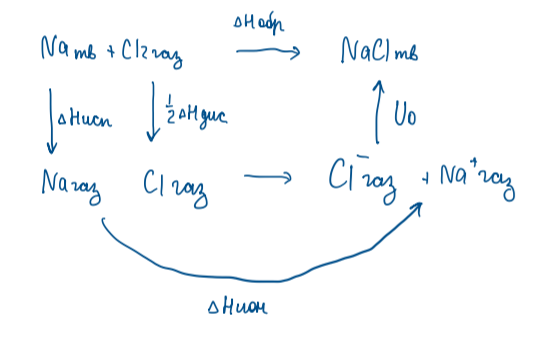
\includegraphics[scale=1]{4.png}}
\end{figure}

\par\smallskip	

Рассмотрим два типа кристаллических решеток для состава $XY$:
$NaCl$ и $CsCl$.

\par\smallskip

\begin{figure}[H]
	\centering
	{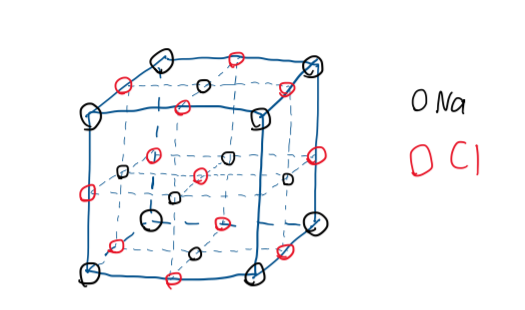
\includegraphics[scale=0.7]{5.png}}
\end{figure}

\par\smallskip

Кристаллы с гранецентрированной кубической решёткой. Восемь
ионов $Na^+$ образуют вершины куба, шесть других в центрах граней.
Анионы хлора располагаются по центрам всех рёбер и в центре
куба. Координационное число обоих ионов равно $6$.

\par\smallskip

\begin{figure}[h]
	\centering
	{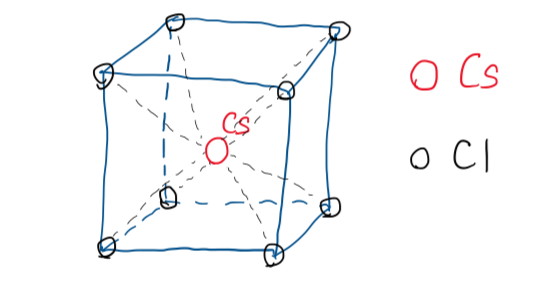
\includegraphics[scale=0.7]{6.png}}
\end{figure}

\par\smallskip

Кристаллы с объёмоцентрированной кубической решёткой. Ионы
хлора занимают $8$ вершин в кубе, а катион цезия располагается в
центре куба, или наоборот. Для обоих ионов координационное
число равно $8$. В кристаллической решётке атом в вершине куба
принадлежит одновременно $8$ ячейкам. 

\par\smallskip

У этих кристаллических решёток различное отношение $\frac{r^-}{r^+}$, если
это отношение находится в том или ином диапазоне, то
предпочтительнее и более устойчивой становится соответствующая
конфигурация:

$$CsCl \;\;\;\;\; 1<\frac{r^-}{r^+}<1.37$$

$$NaCl \;\;\;\;\; 1.37<\frac{r^-}{r^+}<2.44$$


Также у данных структурных типов различается константа
Маделунга и энергия кристаллической решётки. Последняя больше
у $NaCl$.
	
\par\bigskip
\par\bigskip